\documentclass[]{article}
\usepackage{lmodern}
\usepackage{amssymb,amsmath}
\usepackage{ifxetex,ifluatex}
\usepackage{fixltx2e} % provides \textsubscript
\ifnum 0\ifxetex 1\fi\ifluatex 1\fi=0 % if pdftex
  \usepackage[T1]{fontenc}
  \usepackage[utf8]{inputenc}
\else % if luatex or xelatex
  \ifxetex
    \usepackage{mathspec}
  \else
    \usepackage{fontspec}
  \fi
  \defaultfontfeatures{Ligatures=TeX,Scale=MatchLowercase}
\fi
% use upquote if available, for straight quotes in verbatim environments
\IfFileExists{upquote.sty}{\usepackage{upquote}}{}
% use microtype if available
\IfFileExists{microtype.sty}{%
\usepackage{microtype}
\UseMicrotypeSet[protrusion]{basicmath} % disable protrusion for tt fonts
}{}
\usepackage[margin=1in]{geometry}
\usepackage{hyperref}
\PassOptionsToPackage{usenames,dvipsnames}{color} % color is loaded by hyperref
\hypersetup{unicode=true,
            pdftitle={Prioritizing management goals for stream biological integrity within the context of landscape constraints},
            pdfauthor={Marcus W. Beck (marcusb@sccwrp.org), Raphael D. Mazor (raphaelm@sccwrp.org), Scott Johnson (scott@aquaticbioassay.com), Phil Markle (pmarkle@lacsd.org), Joshua Westfall (jwestfall@lacsd.org), Peter D. Ode (peter.ode@wildlife.ca.gov), Ryan Hill (hill.ryan@epa.gov), Eric D. Stein (erics@sccwrp.org)},
            colorlinks=true,
            linkcolor=Maroon,
            citecolor=Blue,
            urlcolor=blue,
            breaklinks=true}
\urlstyle{same}  % don't use monospace font for urls
\usepackage{graphicx,grffile}
\makeatletter
\def\maxwidth{\ifdim\Gin@nat@width>\linewidth\linewidth\else\Gin@nat@width\fi}
\def\maxheight{\ifdim\Gin@nat@height>\textheight\textheight\else\Gin@nat@height\fi}
\makeatother
% Scale images if necessary, so that they will not overflow the page
% margins by default, and it is still possible to overwrite the defaults
% using explicit options in \includegraphics[width, height, ...]{}
\setkeys{Gin}{width=\maxwidth,height=\maxheight,keepaspectratio}
\IfFileExists{parskip.sty}{%
\usepackage{parskip}
}{% else
\setlength{\parindent}{0pt}
\setlength{\parskip}{6pt plus 2pt minus 1pt}
}
\setlength{\emergencystretch}{3em}  % prevent overfull lines
\providecommand{\tightlist}{%
  \setlength{\itemsep}{0pt}\setlength{\parskip}{0pt}}
\setcounter{secnumdepth}{0}
% Redefines (sub)paragraphs to behave more like sections
\ifx\paragraph\undefined\else
\let\oldparagraph\paragraph
\renewcommand{\paragraph}[1]{\oldparagraph{#1}\mbox{}}
\fi
\ifx\subparagraph\undefined\else
\let\oldsubparagraph\subparagraph
\renewcommand{\subparagraph}[1]{\oldsubparagraph{#1}\mbox{}}
\fi

%%% Use protect on footnotes to avoid problems with footnotes in titles
\let\rmarkdownfootnote\footnote%
\def\footnote{\protect\rmarkdownfootnote}

%%% Change title format to be more compact
\usepackage{titling}

% Create subtitle command for use in maketitle
\newcommand{\subtitle}[1]{
  \posttitle{
    \begin{center}\large#1\end{center}
    }
}

\setlength{\droptitle}{-2em}
  \title{Prioritizing management goals for stream biological integrity within the
context of landscape constraints}
  \pretitle{\vspace{\droptitle}\centering\huge}
  \posttitle{\par}
  \author{Marcus W. Beck
(\href{mailto:marcusb@sccwrp.org}{\nolinkurl{marcusb@sccwrp.org}}),
Raphael D. Mazor
(\href{mailto:raphaelm@sccwrp.org}{\nolinkurl{raphaelm@sccwrp.org}}),
Scott Johnson
(\href{mailto:scott@aquaticbioassay.com}{\nolinkurl{scott@aquaticbioassay.com}}),
Phil Markle
(\href{mailto:pmarkle@lacsd.org}{\nolinkurl{pmarkle@lacsd.org}}), Joshua
Westfall
(\href{mailto:jwestfall@lacsd.org}{\nolinkurl{jwestfall@lacsd.org}}),
Peter D. Ode
(\href{mailto:peter.ode@wildlife.ca.gov}{\nolinkurl{peter.ode@wildlife.ca.gov}}),
Ryan Hill
(\href{mailto:hill.ryan@epa.gov}{\nolinkurl{hill.ryan@epa.gov}}), Eric
D. Stein (\href{mailto:erics@sccwrp.org}{\nolinkurl{erics@sccwrp.org}})}
  \preauthor{\centering\large\emph}
  \postauthor{\par}
  \date{}
  \predate{}\postdate{}

\usepackage{lineno}
\linenumbers
\usepackage{setspace}
\linespread{1}
\usepackage{cleveref}
\usepackage{acronym}
\usepackage{booktabs}
\usepackage{multirow}
\acrodef{csci}[CSCI]{California Stream Condition Index}
\acrodef{nhd}[NHD]{National Hydrography Dataset Plus}
\acrodef{pmmi}[pMMI]{predictive multimetric index}
\acrodef{sgr}[SGR]{San Gabriel River}
\acrodef{sgrrmp}[SGRRMP]{San Gabriel River Regional Monitoring Program}

\begin{document}
\maketitle

\section{Abstract}\label{abstract}

Many streams are failing to achieve desired biological condition and
require management decisions to restore designated uses. Some management
goals may be impractical with limited resources, particularly in streams
where large-scale changes on the landscape (e.g., urbanization) impose
constraints on the upper limit of biological integrity. A statewide
landscape model was developed that sets reasonable expectations for
observed conditions within landscape constraints to prioritize
management actions. The model provides a context for what is likely to
be achieved at a given site independent of an actual bioassessment
score. With this approach, sites can be ranked as over- or under-scoring
relative to an expectation that is typical for the observed level of
landscape alteration. We developed a visualization tool to compare
observed bioassessment scores with modelled expectations to rapidly
identify reaches that were scoring better or worse than expected. Using
this tool, a group of regulators, dischargers, stormwater agencies, and
environmental advocates from the San Gabriel River watershed (Los
Angeles County, California) identified regions in the watershed with
consistent patterns in bioassessment scores relative to expectations.
Based on these patterns, they prioritized different management actions
for each region. Sites in both developed and undeveloped areas that
scored below expectations were prioritized for restoration; in contrast,
restoration was not a priority at developed sites where scores were low
but within expected ranges. Sites scoring better than expected were
prioritized for enhanced protection, as well as additional monitoring.
Interactive tools that connect landscape models with observed data can
help set management goals appropriate for stakeholder needs and likely
constraints on biological integrity. These tools can easily be applied
to other locations where biological data are used to assess
environmental condition.

\section{Introduction}\label{introduction}

\begin{itemize}
\item
  Degraded biological condition in streams can occur from individual or
  multiple stressors acting at different scales (Novotny et al.
  \protect\hyperlink{ref-Novotny05}{2005}; Townsend, Uhlmann, and
  Matthaei \protect\hyperlink{ref-Townsend08}{2008}; Leps et al.
  \protect\hyperlink{ref-Leps15}{2015}). Identifying and mitigating
  causes of poor condition requires an understanding of how stressors
  propogate across space and time. Incomplete knowledge on drivers of
  change or high level of uncertainty in how biology is linked to
  drivers can lead to ineffective management actions. Placing bounds on
  effects of known drivers of change can reduce expenses and increase
  assurance of outcomes for targeted management (e.g., varying costs and
  challenges of urban stream restoration (Kenney et al.
  \protect\hyperlink{ref-Kenney12}{2012}; Shoredits and Clayton
  \protect\hyperlink{ref-Shoredits13}{2013}))
\item
  Effective stream management can depend on identification and
  prioritization of sites where activities are expected to have desired
  outcomes. This requires an understanding of how stressors affect
  biological integrity to place bounds on reasonable expectations for
  what is likely to be a possible outcome of a management action. This
  requires identifying biological constraints or limits on the potential
  range of biological conditions. Identifying an appropriate context for
  observed conditions can be used to prioritize. Context can be defined
  by models, expert knowledge, and/or defined value sets.
\item
  We don't have good constraint tools to develop a context of
  expectation of what's possible at a site. This can help prioritize
  locations where management efforts will or will not have the intended
  outcomes. Biological filters act at different scales (Poff
  \protect\hyperlink{ref-Poff97}{1997}) and we can use this information
  to describe an expectation for prioritization that is scale-specific.
  Landscape-level constraints are particularly relevant for
  macroinvertebrate communities in streams (Sponseller, Benfield, and
  Valett \protect\hyperlink{ref-Sponseller01}{2001})
\item
  The goal of this study is to demonstrate application of a landscape
  model to classify and prioritize stream monitoring sites using
  estimated constraints on biological integrity. The model provides an
  estimate of context for biological condition that provides an
  expectation of what is likely to be achieved at a given site relative
  to large-scale drivers of stream health. The model was developed and
  applied to all stream reaches in California. A case study is used to
  demonstrate how the model can be used to classify and prioritize using
  guidance from a regional stakeholder group. Active stakeholder
  involvement was critical in applying the landscape models to define a
  framework for decision-making because priorities varied with
  management objectives.
\end{itemize}

\section{Methods}\label{methods}

\subsection{Study area and data
sources}\label{study-area-and-data-sources}

Landscape models were developed for California using land use data,
stream hydrography, and biological assessments. California covers
424,000 km\(^2\) of land from latitudes 33 to 42\(^\circ\)N that
includes extreme variation in altitude and climate. Temperate
rainforests occur in the north, deserts in the northeast and southeast,
and Mediterranean climates in coastal regions. California's stream
network is approximately 280,000 km in length and covers all of the
major climate zones in the state. A high degree of endemism and
biodiversity occurs in these streams including nearly 4000 species of
vascular plants, macroinvertebrates, and vertebrates that depend on
fresh water during their life history (J. Howard and Revenga
\protect\hyperlink{ref-Howard09}{2000}; J. K. Howard et al.
\protect\hyperlink{ref-Howard15}{2015}). Approximately 30\% of streams
in California are perennial with the remaining as intermittent or
ephemeral for portions of the year. Much of California is publicly owned
and is used heavily for recreation. A large portion of the central
region of the state is agricultural (i.e., Central Valley), whereas
dense areas of urban development are in the southwest (i.e., Los Angeles
and San Diego) and central (San Francisco Bay area) coast areas.
Developed lands increased in California by 38\% from 1973 to 2000
(Sleeter et al. \protect\hyperlink{ref-Sleeter11}{2011}).

\begin{figure}
\centering
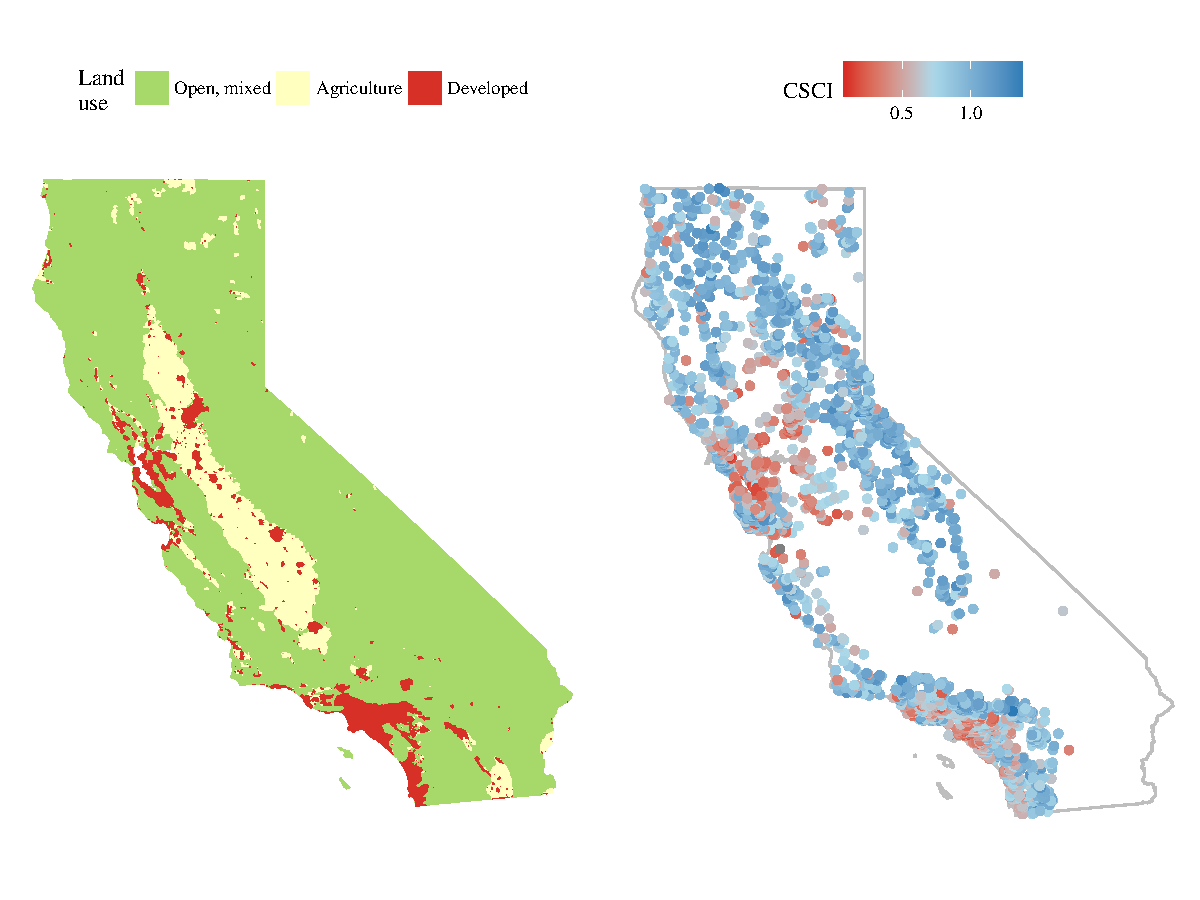
\includegraphics{figs/unnamed-chunk-1-1.pdf}
\caption{test}
\end{figure}

Stream data from the \ac{nhd} (USGS (US Geological Survey)
\protect\hyperlink{ref-USGS14}{2014}) were used to identify reaches in
California for modelling biological integrity. The \ac{nhd} is a surface
water framework that maps drainage networks and associated features
(e.g., streams, lakes, canals, etc.) in the United States. Stream flow
lines in the \ac{nhd} are developed from flow accumulation models that
estimate location of a stream given slope and elevation changes from
existing elevation datasets. As such, flow lines in California represent
both perennial, intermittent, and ephemeral streams that have wide
variation in observed flow throughout the year. Stream reaches
designated in the \ac{nhd} were used as the discrete spatial unit for
modelling biological integrity. A reach is defined as a continuous piece
of surface water with similar hydrologic characteristics (USGS (US
Geological Survey) \protect\hyperlink{ref-USGS14}{2014}). Hydrography
data were combined with landscape metrics available from the StreamCat
Dataset (Hill et al. \protect\hyperlink{ref-Hill16}{2016}) to estimate
land use at the catchment (nearby landscape flowing directly into a
stream) and the entire upstream watershed for each reach. The StreamCat
Dataset was developed specifically for the \ac{nhd} to leverage the
topology of stream connections to estimate cumulative landscape metrics
of all reaches.

The \ac{csci} (Ode et al. \protect\hyperlink{ref-Ode16}{2016}; Mazor et
al. \protect\hyperlink{ref-Mazor16}{2016}) was used as a measure of
biological condition in California streams. Benthic macroinvertebrate
data used to calculate \ac{csci} scores were collected at nearly 3400
sites (6270 with repeat visits) between 2000 and 2016. Field data were
collected during baseflow conditions typically between May and July
following methods in Ode (\protect\hyperlink{ref-Ode07}{2007}). The
\ac{csci} is a predictive index of stream health that compares the
observed taxa and metrics at a site to those expected under reference
conditions. Expected conditions at a site are based on models that
estimate the likely macroinvertebrate community in relation to factors
that naturally influence biology, e.g., watershed size, elevation,
climate, etc. The \ac{csci} score at a site is based on an
observed-to-expected ratio of taxa and a \ac{pmmi} composed of six
individual metrics that describe the structure and function of the
macroinvertebrate community. The index score at a site can vary from 0
to 1.4, with higher values indicating an observed community with less
deviation from reference conditions. Because the index was developed to
minimize the influence of natural gradients, the index scores have
consistent meaning across the state (Reynoldson et al.
\protect\hyperlink{ref-Reynoldson97}{1997}). A threshold score based on
a selected lower percentile of scores (e.g., 10\%) at all reference
sites is used to define nominally low and high scoring sites.

\subsection{Building and validating landscape
models}\label{building-and-validating-landscape-models}

A prediction model of the \ac{csci} was developed to estimate likely
ranges of scores associated with land use gradients. Land use as urban
and agricultural was quantified for the catchment of each stream reach
in California using the StreamCat database (Hill et al.
\protect\hyperlink{ref-Hill16}{2016}). \ac{csci} scores were modelled
using only the estimates of urban and agricultural land use as the
developed portion of the landscape within each stream reach. The model
was incomplete by design to describe scores only in relation to
large-scale constraints on biological condition that are not easily
controlled by management actions or where costs to mitigate are likely
to be excessive. The remainder of the variation in scores not related to
landscape constraints could be attributed to additional, unmeasured
environmental variables that influence stream biointegrity. Deviation of
observed scores from the model predictions were considered diagnostic of
variation not related to landscape effects.

Models were developed using quantile regression forests to estimate
ranges of likely \ac{csci} scores in different landscapes (N.
Meinshausen \protect\hyperlink{ref-Meinshausen06}{2006}; Nicolai
Meinshausen \protect\hyperlink{ref-Meinshausen17}{2017}). Quantile
models evaluate the conditional response across the range of values that
are expected, such as the lower and upper percentiles of the
distribution, as compared to only the mean response with conventional
models (Cade and Noon \protect\hyperlink{ref-Cade03}{2003}). This allows
use of model predictions to describe where bioassessment targets are
unlikely to be met or where streams are unlikely to be impacted by
placing bounds on the range of expectations relative to landscape
constraints. Random forest models also provide robust predictions by
evaluating different subsets of observations from random splits of the
predictor variables. The final predictions are the averaged response
across several models. These models have been used extensively in
bioassessment applications (Carlisle, Falcone, and Meador
\protect\hyperlink{ref-Carlisle09}{2009}; Chen et al.
\protect\hyperlink{ref-Chen14}{2014}; Mazor et al.
\protect\hyperlink{ref-Mazor16}{2016}) and can produce unbiased
estimates that are relatively invariant to noisy relationships or
non-normal distributions (Breiman
\protect\hyperlink{ref-Breiman01}{2001}; Hastie, Tibshirani, and
Friedman \protect\hyperlink{ref-Hastie09}{2009}). Quantile regression
forests were used to predict \ac{csci} scores in each stream reach from
the 5\textsuperscript{th} to the 95\textsuperscript{th} percentile of
expectations at five percent intervals (i.e., 5\textsuperscript{th},
10\textsuperscript{th}, etc.).

Landscape estimates for the catchments of all \ac{nhd} stream reaches in
California were separated into calibration and validation data.

\subsection{San Gabriel River watershed case
study}\label{san-gabriel-river-watershed-case-study}

Stream reach and bioassessment data from the \ac{sgr} watershed in
southern California were used to develop reach classifications, site
performance categories, and management priorities from the landscape
models. A strong land use gradient occurs in the \ac{sgr} watershed.
Headwaters begin in the San Gabriel mountains where the land is
primarily undeveloped or protected for reacreational use, whereas the
lower watershed is in a heavily urbanized region of Los Angeles County.
The San Gabriel river is dammed at four locations for flood control in
the upper watershed and is hydrologically connected to the Los Angeles
river to the west through the Whittier Reservoir in the lower watershed.
Spreading grounds are present in the middle of the watershed for
groundwater recharge during high flow. Nearly all of the stream reaches
in the lower half of the watershed are channelized with concrete or
other reinforcements.

\emph{Figure} SGR watershed

The \ac{sgr} watershed contains a diverse group of stakeholders from
local municipalities, water districts, water quality regulatory
agencies, consulting groups, and non-government organizations.
Collectively, the \ac{sgrrmp} includes stakeholders from these groups
that cooperatively work to increase awareness of issues in the \ac{sgr}
watershed and work to improve coordination of compliance and ambient
monitoring efforts. The stakeholder workgroup included individuals from
the \ac{sgrrmp} with interests in water supply, improvements to water
quality, habitat protection or creation, and storm water permitting.
Individuals were selected for partipation to include a variety of
mangement interests and based on willingness to adopt tools developed
from the landscape models. The stakeholder workgroup met monthly over a
six-month period to discuss model applications and to refine the
interpretation of results. Stakeholder involement was critical for
developing an assessment framework that met the needs of all engaged
parties and ensured that final products were more likely to be
incorporated into formal processes of decision-making.

\subsection{Reach classification, site performance, and
prioritization}\label{reach-classification-site-performance-and-prioritization}

A framework for identifying site priorities for management actions was
developed using a three-step process. First, estimates of the range of
expected \ac{csci} scores at each stream reach in relation to land use
were used to define reach classifications. Second, the relationship
between observed \ac{csci} scores and the reach classifications were
then used to assign a relative performance value for each monitoring
site. Third, site performance categories in relation to reach
classification and bioassessment targets were used to define management
priorities. This framework was developed through close interaction with
the regional stakeholder group to demonstrate how the landscape model
can be used as a management tool given that priorities will vary by
interests and location. As such, the results are provided as a guide to
facilitate decision-making rather than a prescription of targeted
actions to manage stream health.

Identifying site priorities began with defining a classification
framework for stream reaches to identify the possible or likely extent
of biological constraints. Classifications were developed using the
range of \ac{csci} expectations at a reach relative to a chosen
threshold for the \ac{csci} to define nominally low or high scores. The
reach classification was based solely on the intersection of the
\ac{csci} expectations at a reach with chosen \ac{csci} threshold, where
expectations could be below, above, or overlapping the threshold. Stream
reaches with a range of \ac{csci} score expectations entirely below the
thresholds were considered likely constrained, whereas those with
expectations entirely above were considered likely unconstrained.
Reaches with score expectations that included the \ac{csci} thresholds
were considered possibly constrained or possibly unconstrained, where
the distinction was based on location of the median expectation of a
reach relative to the threshold.

\ac{csci} scores from biomonitoring data were used to define performance
of a sample site relative to the stream reach classification. For each
of the four reach classifications (likely constrained, possibly
constrained, possibly unconstrained, and likely unconstrained), the site
performance was defined relative to the bounds of the expected \ac{csci}
scores. This provided a definition of site performance that can be used
to understand the observed score relative to the biological context of a
reach. Sites with observed scores above the upper limit of the reach
expectation (e.g., above the 95\textsuperscript{th} percentile of
expected scores) were considered ``over-performing'' and sites below the
lower limit were ``under-performing''. Sites with \ac{csci} scores
within the range of expectations were as ``expected''.

\emph{Figure} classification and performance

Site performance categories were further split relative to location to
the selected \ac{csci} threshold. This final split was created with the
intent that description of site scores relative to a defined threshold
(e.g., impairment threshold or restoration target) should also be
considered. Specifically, a fourth category of site performance for each
reach classifcation was added to define a site as above or below the
threshold. For a likely unconstrained reach, underperforming sites below
the minimum expected score were additionally defined as being above or
below the \ac{csci} threshold. Similarly, overperforming sites above the
maximum expected score in a likely constrained reach were additionally
defined as being below or above the \ac{csci} threshold. For possibly
constrained and possibly unconstrained reaches, sites that were
performing as expected were addtionally defined as being below or above
the \ac{csci} threshold. In total, sixteen site types were defined for
the three reach classification and three site performance
classifications (\cref{tab:typetab}).

\begin{table}[!tbp]
\caption{Possible site types based on stream reach classification, site performance, and observed \ac{csci} score. The observed score column describes where a \ac{csci} score is observed relative to the lower and upper percentiles (e.g., 5\textsuperscript{th} and 95\textsuperscript{th}) of expected scores for a reach and the chosen \ac{csci} threshold (e.g., 10\textsuperscript{th} percentile of scores at reference sites or 0.79) for nominally low or high values.\label{tab:typetab}} 
\begin{center}
\begin{tabular}{llll}
\hline\hline
\multicolumn{1}{l}{Reach expectation}&\multicolumn{1}{c}{Site performance}&\multicolumn{1}{c}{Observed score}&\multicolumn{1}{c}{Type}\tabularnewline
\hline
\textbf{likely unconstrained}&over scoring&$\geq$ 95\textsuperscript{th}&1\tabularnewline
&expected&5\textsuperscript{th} to 95\textsuperscript{th}&2\tabularnewline
&under scoring&0.79 to 5\textsuperscript{th}&3\tabularnewline
&under scoring&\textless  0.79&4\tabularnewline
\textbf{possibly unconstrained}&over scoring&$\geq$ 95\textsuperscript{th}&5\tabularnewline
&expected&0.79 to 95\textsuperscript{th}&6\tabularnewline
&expected&5\textsuperscript{th} to 0.79&7\tabularnewline
&under scoring&\textless  5\textsuperscript{th}&8\tabularnewline
\textbf{possibly constrained}&over scoring&$\geq$ 95\textsuperscript{th}&9\tabularnewline
&expected&0.79 to 95\textsuperscript{th}&10\tabularnewline
&expected&5\textsuperscript{th} to 0.79&11\tabularnewline
&under scoring&\textless  5\textsuperscript{th}&12\tabularnewline
\textbf{likely constrained}&over scoring&$\geq$ 0.79&13\tabularnewline
&over scoring&95\textsuperscript{th} to 0.79&14\tabularnewline
&expected&5\textsuperscript{th} to 95\textsuperscript{th}&15\tabularnewline
&under scoring&\textless  5\textsuperscript{th}&16\tabularnewline
\hline
\end{tabular}\end{center}
\end{table}

Each site type was used to define a priority as a demonstration of how
results from the landscape model can help achieve different stream
management objectives. This final process relied exclusively on feedback
from the stakeholder group that represented interests in monitoring,
regulation, restoration, and protection. Priorities for each site type
were defined accordingly with the expectation that site types will have
different meanings for prioritization given the interest. Stakeholders
from each sector were tasked with identifying their relevant priorities
by ranking each site type from high to low priority using a blank
template for reference (Figure). A brief description of the rationale
for a site priority was also requested with the feedback.

\emph{Figure} Site types template figure for prioritization

\emph{Figure} App screenshot

\subsection{Sensitivity analyses}\label{sensitivity-analyses}

Stream reach classifications and site performance categories depend on
the range of score expectations from the landscape model and the
\ac{csci} threshold for defining nominally low or high scores. This
framework for identifying priorities was developed to allow flexibility
in how the model could be applied. First, the framework can accommodate
degrees of certainty in the model by allowing variation in the range of
scores that are used to define a stream reach classification. The
5\textsuperscript{th} and 95\textsuperscript{th} percentile of expected
scores at a reach are used as a default range in which a high degree of
certainty in the model output is assumed. The ability to reduce this
range (e.g., 25\textsuperscript{th} to 75\textsuperscript{th}
percentile) to assume less certainty in the model is provided. The
\ac{csci} threshold can also be changed to assess effects of relaxing or
increasing flexibility in a potential definition of a regulatory
standard. A threshold of 0.79 is used by default as a measure of the
10\textsuperscript{th} percentile of scores at all reference
(non-impacted) sites that were used to calibrate the \ac{csci} index.
This value can be increased to examine effects of a more stringent
threshold or decreased for a more relaxed threshold. The combined
effects of changing both the certainty in the model and the \ac{csci}
threshold were evaluated to estimate the changes in stream miles in each
classification and the number of sites in each priority type.

\subsection{Unclassified reaches}\label{unclassified-reaches}

Finally, some stream reaches were unclassifed following application of
the landscape model to the statewide hydrography dataset. Unclassified
reaches occurred when insufficient data in the StreamCat database were
available to estimate \ac{csci} predictions or if a stream catchment
basin could not be defined for a particular reach. The latter was more
common, particularly in developed areas where engineered channels or
agricultural ditches were hydrologically removed from the natural stream
network. Overall, unclassified reaches were not common in the statewide
dataset but they may have regional importance depending on needs of
local management groups. A preliminary approach for assigning biological
expectations to unclassified reaches is demonstrated for `typically'
urban and agriculture reaches that relies on the range of expectations
for reaches with similar land use by region.

\section{Results}\label{results}

\subsection{State-wide patterns}\label{state-wide-patterns}

\begin{itemize}
\item
  Where does the model perform well, how does performance vary with
  validation and calibration datasets.
\item
  What is the consistency of patterns? For example, percent stream miles
  as xyz by PSA.
\end{itemize}

\emph{Figure} Statewide map.

\subsection{Case study}\label{case-study}

\begin{itemize}
\item
  Extent, classification, prioritization
\item
  Relationships with environmental variables for
  constrained/unconstrained locations. Maybe apply to
  hardened/non-hardened reaches in constrained locations.
\end{itemize}

\emph{Figure} Summary of extent of reach classification, site
performance, selected examples

\emph{Tables} Priority table(s) from stakeholder group

\subsection{Sensitivity analysis}\label{sensitivity-analysis}

\begin{itemize}
\item
  Statewide results - reach classification, site performance
\item
  SGR application - where do priorities change? Do overall patterns
  remain?
\end{itemize}

\emph{Table} Sensitivity results

\subsection{Unclassified reaches}\label{unclassified-reaches-1}

\begin{itemize}
\item
  Extent of typical ag, typical urban statewide
\item
  Framework for assigning unclassified reach to a class
\item
  Statewide patterns, SGR patterns
\end{itemize}

\emph{Table} Summary by location

\section{Discussion}\label{discussion}

\begin{itemize}
\tightlist
\item
  What is the value of identifying constrained channels?

  \begin{itemize}
  \tightlist
  \item
    Use of more data to develop context of assessment
  \item
    Targeted management for desired outcomes
  \end{itemize}
\item
  What is useful about our approach compared to alternatives?

  \begin{itemize}
  \tightlist
  \item
    Field-based methods to identify modified channels vs.~landscape
    modelling
  \item
    (Hill et al. \protect\hyperlink{ref-Hill17}{2017}) as alternative
    example of landscape modelling
  \item
    Related directly to biological condition and regulatory standards
  \item
    Results are widely corraborated by other landscape studies - land
    use is big determinant of macroinvert assemblage
  \end{itemize}
\item
  What contributed to our success in defining priorities?

  \begin{itemize}
  \tightlist
  \item
    Stakeholder involvement guided process, contributed to achieving
    goals
  \item
    An interactive/iterative approach was used - we provided tools to
    facilitate (web apps) and we did not assume priorities
  \end{itemize}
\item
  Caveats of our aproach

  \begin{itemize}
  \tightlist
  \item
    What do priorities really mean? Depends on your interests, needs,
    values, etc.
  \item
    Constrained may not always mean constrained - CSCI vs other
    biological indicators
  \item
    Site-specific approaches are warranted in certain cases
  \item
    Changing certainty or CSCI treshold - mechanistic effects and
    implications. Don't cook the books.
  \end{itemize}
\item
  Future work

  \begin{itemize}
  \tightlist
  \item
    Link with engineered channels study
  \item
    Priorities statewide, application to larger regions possible
    (national-scale)
  \end{itemize}
\end{itemize}

\section{Supplement}\label{supplement}

Online application.

\section*{References}\label{references}
\addcontentsline{toc}{section}{References}

\hypertarget{refs}{}
\hypertarget{ref-Breiman01}{}
Breiman, L. 2001. ``Random Forests.'' \emph{Machine Learning} 45: 5--32.

\hypertarget{ref-Cade03}{}
Cade, B. S., and B. R. Noon. 2003. ``A Gentle Introduction to Quantile
Regression for Ecologists.'' \emph{Frontiers in Ecology and the
Environment} 1 (8): 412--20.

\hypertarget{ref-Carlisle09}{}
Carlisle, D. M., J. Falcone, and M. R. Meador. 2009. ``Predicting the
Biological Condition of Streams: Use of Geospatial Indicators of Natural
and Anthropogenic Characteristics of Watersheds.'' \emph{Environmental
Monitoring and Assessment} 151 (1-4): 143--60.
doi:\href{https://doi.org/10.1007/s10661-008-0256-z}{10.1007/s10661-008-0256-z}.

\hypertarget{ref-Chen14}{}
Chen, K., R. M. Hughes, S. Xu, J. Zhang, D. Cai, and B. Wang. 2014.
``Evaluating Performance of Macroinvertebrate-Based Adjusted and
Unadjusted Multi-Metric Indices (MMI) Using Multi-Season and Multi-Year
Samples.'' \emph{Ecological Indicators} 36: 142--51.
doi:\href{https://doi.org/10.1016/j.ecolind.2013.07.006}{10.1016/j.ecolind.2013.07.006}.

\hypertarget{ref-Hastie09}{}
Hastie, T., R. Tibshirani, and J. Friedman. 2009. \emph{The Elements of
Statistical Learning: Data Mining, Inference, and Prediction}. 2nd ed.
New York: Springer.

\hypertarget{ref-Hill17}{}
Hill, R. A., E. W. Fox, S. G. Leibowitz, A. R. Olsen, D. J. Thornbrugh,
and M. H. Weber. 2017. ``Predictive Mapping of the Biotic Condition of
Conterminous U.S. Rivers and Streams.'' \emph{Ecological Applications}
27 (8): 2397--2415.
doi:\href{https://doi.org/10.1002/eap.1617}{10.1002/eap.1617}.

\hypertarget{ref-Hill16}{}
Hill, R. A., M. H. Weber, S. G. Leibowitz, A. R. Olsen, and D. J.
Thornbrugh. 2016. ``The Stream-Catchment (StreamCat) Dataset: A Database
of Watershed Metrics for the Conterminous United States.'' \emph{Journal
of the American Water Resources Assocation} 52: 120--28.
doi:\href{https://doi.org/10.1111/1752-1688.12372}{10.1111/1752-1688.12372}.

\hypertarget{ref-Howard15}{}
Howard, J. K., K. R. Klausmeyer, K. A. Fesenmyer, J. Furnish, T.
Gardali, T. Grantham, J. V. E. Katz, et al. 2015. ``Patterns of
Freshwater Species Richness, Endemism, and Vulnerability in
California.'' \emph{PLOS ONE} 10 (7): e0130710.
doi:\href{https://doi.org/10.1371/journal.pone.0130710}{10.1371/journal.pone.0130710}.

\hypertarget{ref-Howard09}{}
Howard, J., and C. Revenga. 2000. ``California's Freshwater Biodiveristy
in a Continental Context. Science for Conservation Technical Brief
Series.'' San Francisco, CA: The Nature Conservancy of California.

\hypertarget{ref-Kenney12}{}
Kenney, M. A., P. R. Wilcock, B. F. Hobbs, N. E. Flores, and D. C.
Martínez. 2012. ``Is Urban Stream Restoration Worth It?'' \emph{Journal
of the American Water Resources Association} 48 (3): 603--15.
doi:\href{https://doi.org/10.1111/j.1752-1688.2011.00635.x}{10.1111/j.1752-1688.2011.00635.x}.

\hypertarget{ref-Leps15}{}
Leps, M., J. D. Tonkin, V. Dahm, P. Haase, and A. Sundermann. 2015.
``Disentangling Environmental Drivers of Benthic Invertebrate
Assemblages: The Role of Spatial Scale and Riverscape Heterogeneity in a
Multiple Stressor Environment.'' \emph{Science of the Total Environment}
536: 546--56.
doi:\href{https://doi.org/10.1016/j.scitotenv.2015.07.083}{10.1016/j.scitotenv.2015.07.083}.

\hypertarget{ref-Mazor16}{}
Mazor, R. D., A. C. Rehn, P. R. Ode, M. Engeln, K. C. Schiff, E. D.
Stein, D. J. Gillett, D. B. Herbst, and C. P. Hawkins. 2016.
``Bioassessment in Complex Environments: Designing an Index for
Consistent Meaning in Different Settings.'' \emph{Freshwater Science} 35
(1): 249--71.

\hypertarget{ref-Meinshausen06}{}
Meinshausen, N. 2006. ``Quantile Regression Forests.'' \emph{Journal of
Machine Learning Research} 7: 983--99.

\hypertarget{ref-Meinshausen17}{}
Meinshausen, Nicolai. 2017. \emph{QuantregForest: Quantile Regression
Forests}. \url{https://CRAN.R-project.org/package=quantregForest}.

\hypertarget{ref-Novotny05}{}
Novotny, V., A. Bartosová, N. O'Reilly, and T. Ehlinger. 2005.
``Unlocking the Relationship of Biotic Integrity of Impaired Waters to
Anthropogenic Stresses.'' \emph{Water Research} 39 (1): 184--98.
doi:\href{https://doi.org/10.1016/j.watres.2004.09.002}{10.1016/j.watres.2004.09.002}.

\hypertarget{ref-Ode07}{}
Ode, P. R. 2007. ``Standard Operating Procedures for Collecting Benthic
Macroinvertebrate Samples and Associated Physical and Chemical Data for
Ambient Bioassessment in California.'' Surface Water Ambient Monitoring
Program. Sacramento, CA.

\hypertarget{ref-Ode16}{}
Ode, P. R., A. C. Rehn, R. D. Mazor, K. C. Schiff, E. D. Stein, J. T.
May, L. R. Brown, et al. 2016. ``Evaluating the Adequacy of a
Reference-Site Pool for Ecological Assessments in Environmentally
Complex Regions.'' \emph{Freshwater Science} 35 (1): 237--48.

\hypertarget{ref-Poff97}{}
Poff, N. L. 1997. ``Landscape Filters and Species Traits: Towards
Mechanistic Understanding and Prediction in Stream Ecology.''
\emph{Journal of the North American Benthological Society} 16 (2):
391--409.

\hypertarget{ref-Reynoldson97}{}
Reynoldson, T. B., R. H. Norris, V. H. Resh, K. E. Day, and D. M.
Rosenberg. 1997. ``The Reference Condition: A Comparison of Multimetric
and Multivariate Approaches to Assess Water-Quality Impairment Using
Benthic Macroinvertebrates.'' \emph{Journal of the North American
Benthological Society} 16 (4): 833--52.

\hypertarget{ref-Shoredits13}{}
Shoredits, A. S., and J. A. Clayton. 2013. ``Assessing the Practice and
Challenges of Stream Restoration in Urbanized Environments of the USA.''
\emph{Geography Compass} 7 (5): 358--72.
doi:\href{https://doi.org/10.1111/gec3.12039}{10.1111/gec3.12039}.

\hypertarget{ref-Sleeter11}{}
Sleeter, B. M., T. S. Wilson, C. E. Soulard, and J. Liu. 2011.
``Estimation of the Late Twentieth Century Land-Cover Change in
California.'' \emph{Environmental Monitoring and Assessment} 173 (1-4):
251--66.
doi:\href{https://doi.org/10.1007/s10661-010-1385-8}{10.1007/s10661-010-1385-8}.

\hypertarget{ref-Sponseller01}{}
Sponseller, R. A., E. F. Benfield, and H. M. Valett. 2001.
``Relationships Between Land Use, Spatial Scale and Stream
Macroinvertebrate Communities.'' \emph{Freshwater Biology} 46 (10):
1409--24.
doi:\href{https://doi.org/10.1046/j.1365-2427.2001.00758.x}{10.1046/j.1365-2427.2001.00758.x}.

\hypertarget{ref-Townsend08}{}
Townsend, C. R., S. S. Uhlmann, and C. D. Matthaei. 2008. ``Individual
and Combined Responses of Stream Ecosystems to Multiple Stressors.''
\emph{Journal of Applied Ecology} 45 (6): 1810--9.
doi:\href{https://doi.org/10.1111/j.1365-2664.2008.01548.x}{10.1111/j.1365-2664.2008.01548.x}.

\hypertarget{ref-USGS14}{}
USGS (US Geological Survey). 2014. ``National Hydrography Dataset
available on the World Wide Web.''


\end{document}
